%% LyX 2.1.2 created this file.  For more info, see http://www.lyx.org/.
%% Do not edit unless you really know what you are doing.
\documentclass[english]{beamer}
\usepackage{mathptmx}
\usepackage[T1]{fontenc}
\usepackage[latin9]{inputenc}
\usepackage{amsmath}
\usepackage{amssymb}
\usepackage{mathrsfs}
\usepackage{listings}
\usepackage{stmaryrd}
\usepackage{enumitem}
\usepackage{changepage}
\usepackage{diagbox}
\usepackage{pifont}
\usepackage{caption}
\usepackage{float}
\usepackage{csquotes}
\usepackage[backend=biber,
style=numeric,
%style=alphabetic,
%style=reading,
sorting=ynt
]{biblatex}
\addbibresource{Thesis_Proposal_Seminar_Presentation.bib}

\usefonttheme{professionalfonts}

\lstset{
  mathescape,
  backgroundcolor=\color{gray!10},  
  basicstyle=\small,
  columns=fullflexible,
  breakatwhitespace=false,      
  breaklines=true,                
  captionpos=b,                    
  commentstyle=\color{mygreen}, 
  extendedchars=true,              
  frame=single,                   
  keepspaces=true,             
  keywordstyle=\color{black},      
  language=c++,                 
  numbers=none,                
  numbersep=5pt,                   
  numberstyle=\tiny\color{blue}, 
  rulecolor=\color{black},        
  showspaces=false,               
  showstringspaces=false,
  showtabs=false,                 
  stepnumber=5,                  
  stringstyle=\color{mymauve},   
  tabsize=3,                      
  title=\lstname                
}

\makeatletter
%%%%%%%%%%%%%%%%%%%%%%%%%%%%%% Textclass specific LaTeX commands.
 % this default might be overridden by plain title style
 \newcommand\makebeamertitle{\frame{\maketitle}}%
 % (ERT) argument for the TOC
 \AtBeginDocument{%
   \let\origtableofcontents=\tableofcontents
   \def\tableofcontents{\@ifnextchar[{\origtableofcontents}{\gobbletableofcontents}}
   \def\gobbletableofcontents#1{\origtableofcontents}
   \renewcommand{\labelitemi}{$\bullet$}
   \renewcommand{\labelitemii}{$\circ$}
 }

\renewenvironment{quote}[1][1em]
  {\begin{adjustwidth}{#1}{#1}}
  {\end{adjustwidth}}

%%%%%%%%%%%%%%%%%%%%%%%%%%%%%% User specified LaTeX commands.
\usetheme{Warsaw}
% or ...

\setbeamercovered{transparent}
% or whatever (possibly just delete it)

\makeatother

\usepackage{babel}
\newcommand\mytextbullet{\leavevmode%
\usebeamertemplate{itemize item}\hspace{.5em}}

\newtheorem{thm}[theorem]{Theorem}
\newtheorem{defi}[theorem]{\translate{Definition}}
\newtheorem{lem}[theorem]{\translate{Lemma}}
\newtheorem{question}[theorem]{\translate{Question}}
\newtheorem{questions}[theorem]{\translate{Questions}}
\newtheorem{proposition}[theorem]{\translate{Proposition}}
\theoremstyle{example}
\newtheorem{approach}[theorem]{\translate{Approach}}
\newtheorem{conjecture}[theorem]{\translate{Conjecture}}
\newtheorem{difficulty1}[theorem]{Reformulate: $\bar{N}_0 \in D^*$}
\newtheorem{difficulty2}[theorem]{Reformulate: stationarity of members of $\mathcal{P}(\omega_1^V) \cap N_{\omega_1^V} \setminus I_{\omega_1^V}$}
\newtheorem{answer}[theorem]{Answers}
\newtheorem{conclusion}[theorem]{Conclusion}
\newtheorem{observation}[theorem]{Observation}


\begin{document}





\title[Generation as Computation]{Generation as Computation}
\subtitle{Generalised Computation in the Set-theoretic Universe and Beyond \\ (Thesis Proposal)}
\author{Desmond Lau}
\institute{National University of Singapore}


\makebeamertitle


%\pgfdeclareimage[height=0.5cm]{institution-logo}{institution-logo-filename}
%\logo{\pgfuseimage{institution-logo}}



\AtBeginSubsection[]{%
  \frame<beamer>{ 
    \frametitle{Outline}   
    \tableofcontents[currentsubsection] 
  }
}



%\beamerdefaultoverlayspecification{<+->}
\begin{frame}{Outline}


\tableofcontents{}


\end{frame}

\section{Introduction}

\subsection{Background: Infinitary Computation}

\subsection[Background: \textit{Formulas as Programs}]{Background: Formulas as Programs}

\subsection{Overview}

\begin{frame}{Overview Chart}
\begin{figure}[!htp]
    \centering
    \centerline{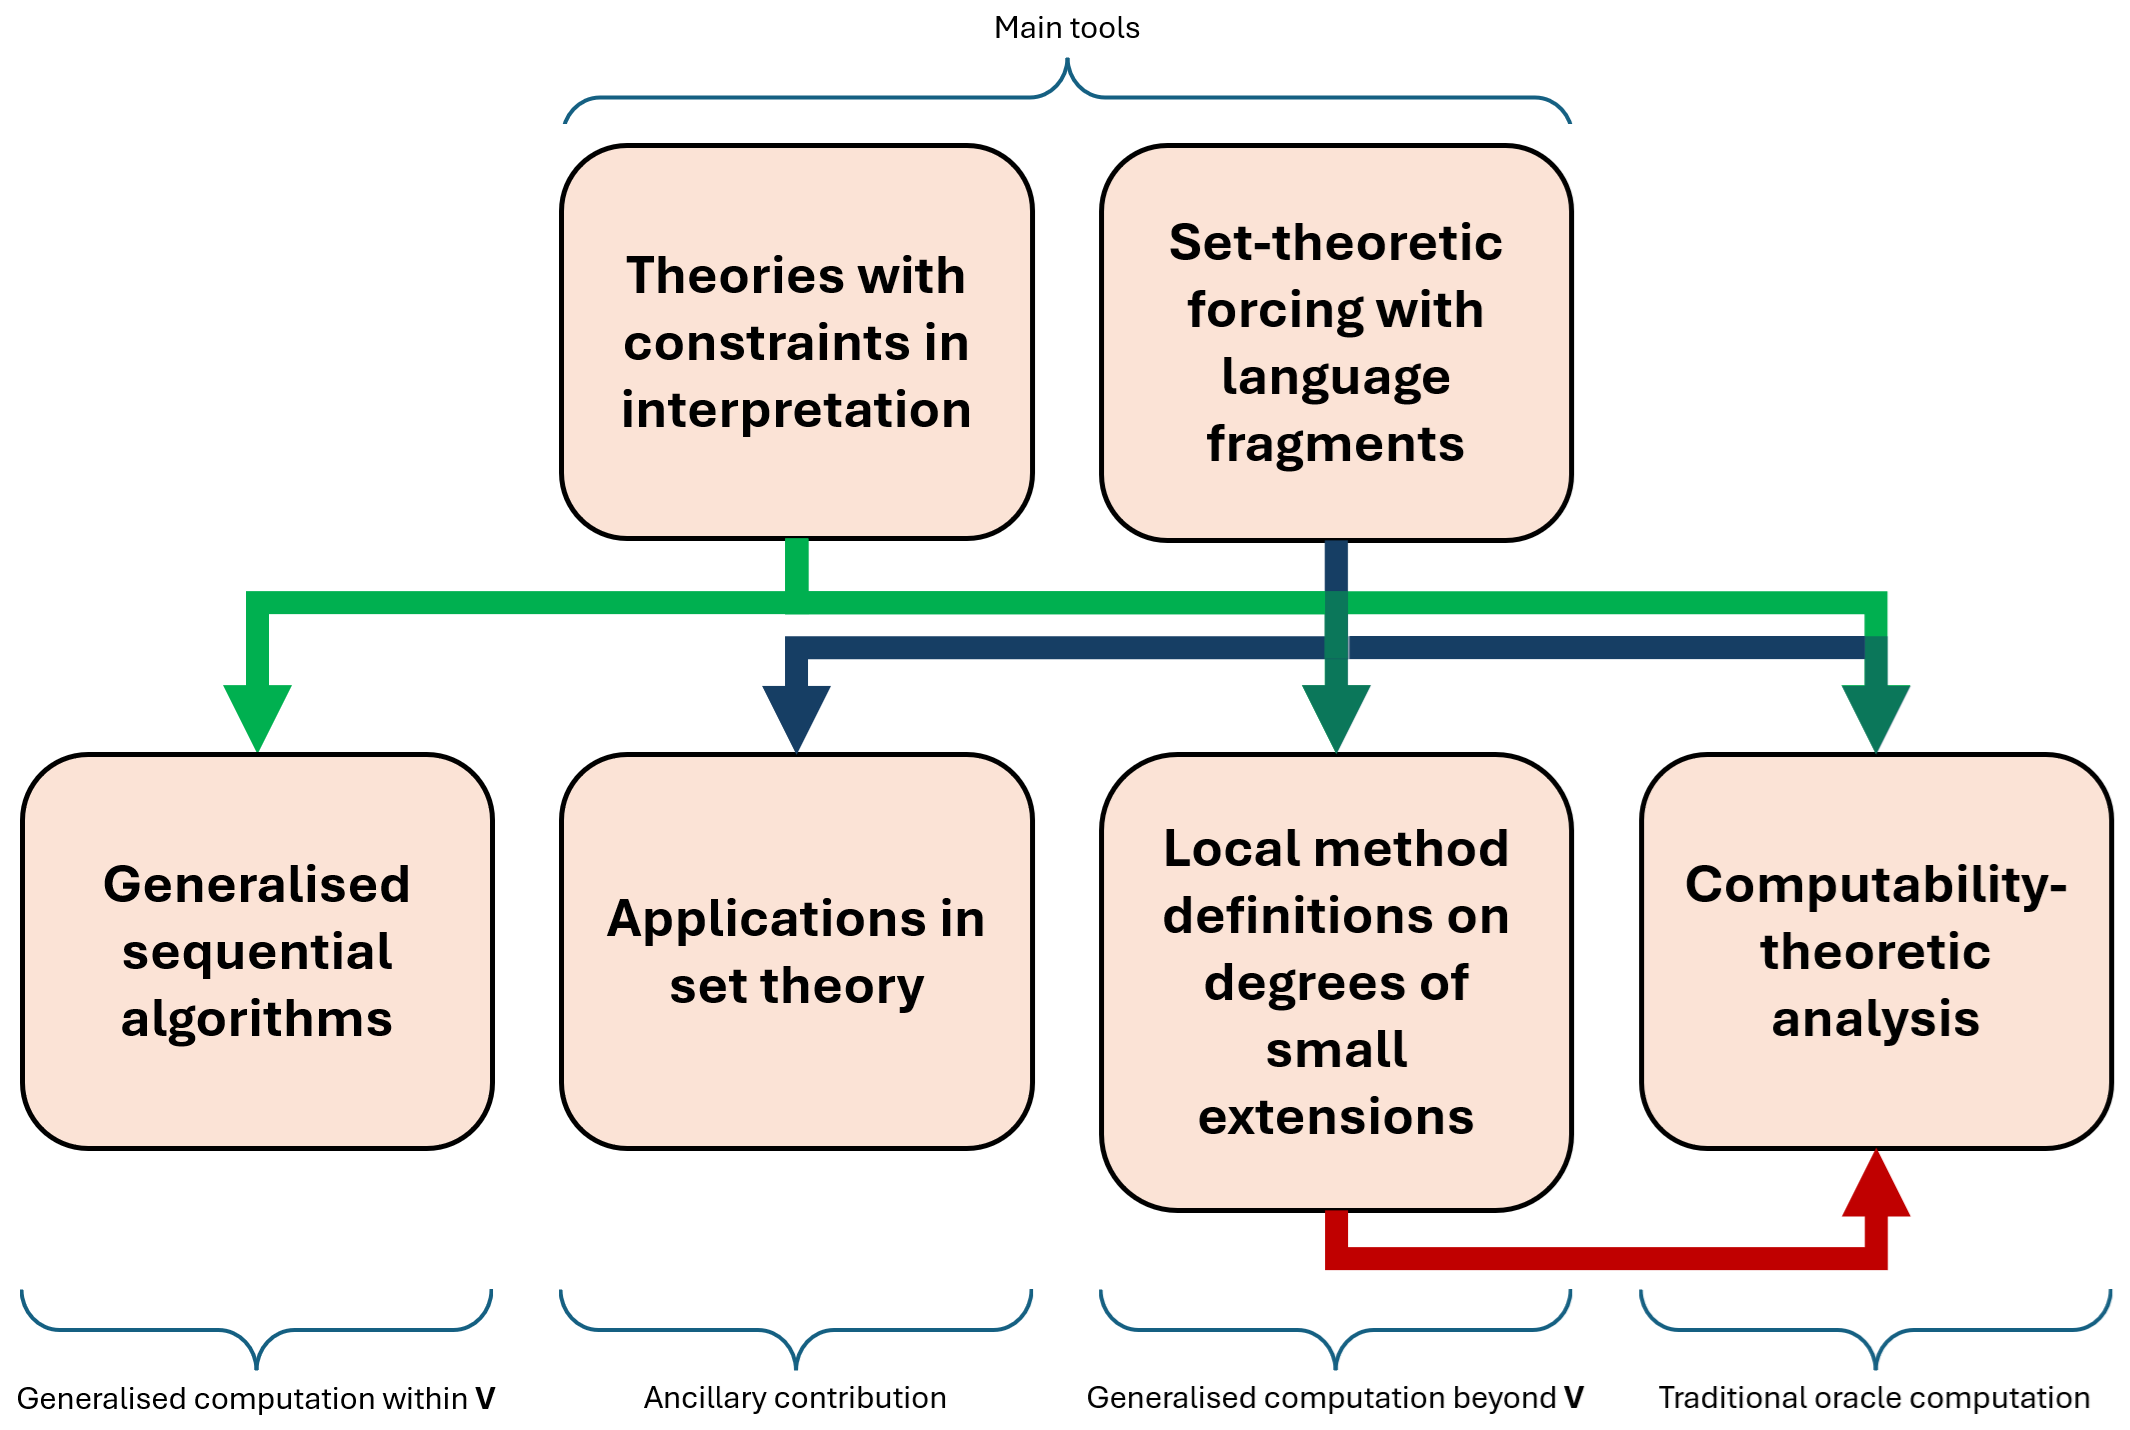
\includegraphics[width=\textwidth]{Overview_Chart_Presentation.png}}
    \label{overview}
\end{figure}
\end{frame}

\section[Generalised Computation Within $V$]{Generalised Computation Within V}

\subsection{Generalised Sequential Algorithms}

\begin{frame}{Upshot}
\pause{}
\begin{itemize}
    \item All reasonable transfinite abstract algorithms are expressible as GSeqAPs. 
    \pause{}
    \item Here \textit{reasonable} means satisfying the boundedness and locality conditions.
\end{itemize}
\end{frame}

\subsection{Comparisons with Other Notions}

\begin{frame}{Summary Table}
\pause{}
In the following table we compare various relative computability relations when they are restricted to subsets of admissible ordinals $\alpha$. \pause{} 
\bigskip
\begin{table}[!htp]
    \footnotesize
    \centering
    \begin{tabular}{|l||*{4}{c|}}\hline
        \backslashbox[90pt]{\scriptsize Property}{\scriptsize Relation}
        &\makebox[4em]{$\leq_{\alpha}$}&\makebox[4em]{$\preceq_{\alpha}$}
        &\makebox[2em]{$\leq^P_{\alpha}$}&\makebox[2em]{$\leq^{P, s}_{\alpha}$}\\\hline\hline
        Oracle-analogue? & \ding{51} & \ding{51} & \ding{55} & \ding{55} \\\hline
        Transitive? & \ding{51} & \ding{55} & \ding{51} & \ding{51} \\\hline
        Upward consistent? & \ding{55} & \ding{51} & \ding{51} & \ding{51} \\\hline
        Appears in$\dots$ & $\alpha$-recursion & $\alpha$-computability &&\\\hline
    \end{tabular}
\end{table}
\end{frame}

\section[Generalised Computation Beyond $V$]{Generalised Computation Beyond V}

\subsection{Degrees of Small Extensions}

\begin{frame}{Generators over $V$}
\pause{}
\begin{itemize}
    \item Going further in the direction of generalised computation, can we maintain the definition of constructibility degrees, but swop $L$ for $V$?
    \pause{}
    \item In essence, we want to group sets outside $V$ based on their power as generators over $V$.
\end{itemize}
\end{frame}

\begin{frame}{The Meta-theory}
\pause{}
\begin{itemize}
    \item What do we mean by ``sets outside $V$''? 
    \pause{}
    \item Step out of $V$ and treat $V$ as a countable transitive model of $\mathrm{ZFC}$ (henceforth denoted CTM).
    \pause{}
    \item Look at those sets that can be adjoined to $V$ to give a nice CTM.
    \pause{}
    \item What do we mean by ``a nice CTM''?
\end{itemize}
\end{frame}

\begin{frame}{Outer Models}
\pause{}
\begin{itemize}
    \item Let $U_1$ and $U_2$ be CTMs. $U_2$ is an outer model of $U_1$ iff
    \pause{}
    \begin{itemize}
        \item $U_1 \subset U_2$, and
        \pause{}
        \item $ORD^{U_1} = ORD^{U_2}$.
    \end{itemize}
    \pause{}
    \item The binary relation ``being an outer model of'' is transitive.
\end{itemize}
\pause{}
\begin{definition}
Let $V$ be a CTM. The \emph{outward multiverse centred at} $V$ is the set
\pause{}
\begin{equation*}
    \mathbf{M}(V) := \{W : W \text{ is an outer model of } V\} \text{.}
\end{equation*}
\end{definition}
\end{frame}

\begin{frame}{Small Extensions}
\pause{}
\begin{definition}[L.]
    Let $U_1$ and $U_2$ be CTMs. $U_2$ is a \emph{small extension of} $U_1$ iff
    \pause{}
    \begin{itemize}
        \item $U_2$ is an outer model of $U_1$, and
        \pause{}
        \item there is $x \in U_2$ such that $U_2$ is the smallest outer model of $U_1$ containing $x$.
    \end{itemize}
    \pause{}
    In this case we call $x$ a \emph{generator of} $U_2$ \emph{over} $U_1$, and denote $U_2$ as $U_1[x]$.
\end{definition}
\pause{}
The binary relation ``being a small extension of'' is transitive.
\pause{}
\begin{definition}
Let $V$ be a CTM. The \emph{small outward multiverse centred at} $V$ is the set
\pause{}
\begin{equation*}
    \mathbf{M}_{S}(V) := \{W : W \text{ is a small extension of } V\} \text{.}
\end{equation*}
\end{definition}
\end{frame}

\begin{frame}{Assorted Multiversal Properties}
\pause{}
Due to Jensen's result on ``coding the universe'', we have the following theorem.
\pause{}
\begin{theorem}[Jensen]
Given a CTM $V$, $(\mathbf{M}_{S}(V), \subset)$ is a cofinal subposet of $(\mathbf{M}(V), \subset)$.
\end{theorem}
\end{frame}

\begin{frame}{Assorted Multiversal Properties}
\pause{}
The next proposition is easy to see.
\pause{}
\begin{proposition}
Let $V$ be a CTM. Then
\pause{}
\begin{equation*}
   \mathbf{M}_{S}(V) = \{V[x] : x \in \bigcup \mathbf{M}(V) \cap \bigcup \{\mathcal{P}(\alpha) : \alpha \in ORD^V\}\} \text{.}
\end{equation*}
\end{proposition}
\end{frame}

\begin{frame}{Assorted Multiversal Properties}
\pause{}
\begin{itemize}
    \item Given a CTM $V$, we want to define a degree structure on generators of small extensions of $V$, analogous to the constructibility degrees on sets in $V$.
    \pause{}
    \item By the previous proposition, it suffices to consider equivalence classes arising from the natural reducibility relation on
    \pause{}
    \begin{equation*}
        \mathcal{G}(V) := \bigcup \mathbf{M}(V) \cap \bigcup \{\mathcal{P}(\alpha) : \alpha \in ORD^V\} \text{.}
    \end{equation*}
\end{itemize}
\end{frame}

\begin{frame}{Degrees over $V$}
\pause{}
\begin{itemize}
    \item Specifically, define the binary relation $\leq^S$ on $\mathcal{G}(V)$ by
    \pause{}
    \begin{equation*}
        \vspace{-\baselineskip + 5pt}
        x \leq^S y \iff V[x] \subset V[y] \text{.}
        \vspace{-\baselineskip + 5pt}
    \end{equation*}
    \pause{}
    \item $\leq^S$ partially orders $\mathcal{G}(V)$, so we can define the equivalence relation $\equiv^S$ the usual way. 
    \pause{}
    \item Call $(\mathcal{G} / \equiv^S, \leq^S / \equiv^S)$ the \emph{degrees of small extensions of} $V$ with its standard partial ordering.
    \pause{}
    \item Observe that \vspace{-\baselineskip + 5pt} 
    \begin{equation*}
        \vspace{-\baselineskip + 5pt} 
        (\{\text{small extensions of } V\}, \subset) \cong (\mathcal{G} / \equiv^S, \leq^S / \equiv^S) \text{,}
    \end{equation*}
    \pause{}
    so ``small extension(s)'' and ``degree(s) of small extensions'' are often used interchangeably.
\end{itemize}
\end{frame}

\begin{frame}{Drawing Parallels}

\end{frame}

\begin{frame}{Drawing Parallels}
\begin{figure}[!ht]
    \centering
    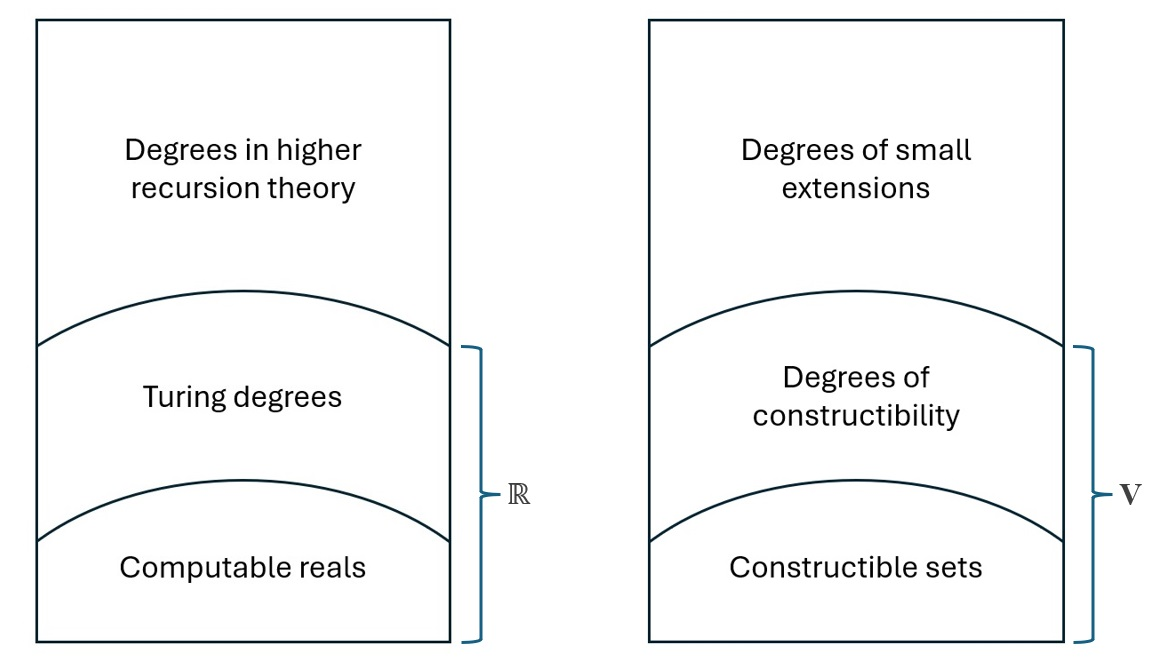
\includegraphics[height = 170pt, keepaspectratio=1]{analogy.jpg}
    \captionsetup{width=0.9\textwidth, format=hang}
    \caption{comparison between conventional notions of relative computability (left) and our generalised notions (right).}
    \label{analogy}
\end{figure}
\end{frame}

\begin{frame}{Multiverse of Generic Extensions}
\pause{}
\begin{definition}
Let $V$ be a CTM. The \emph{outward generic multiverse centred at} $V$ is the set
\pause{}
\begin{equation*}
    \mathbf{M}_{F}(V) := \{W : W \text{ is a forcing extension of } V\} \text{.}
\end{equation*}
\end{definition}
\pause{}
The following fact is basic.
\pause{}
\begin{fact}
Every generic extension is a small extension. Equivalently, 
\begin{equation*}
    \mathbf{M}_{F}(V) \subset \mathbf{M}_{S}(V) \text{.}
\end{equation*}
\end{fact}
\end{frame}

\begin{frame}{Multiverse of Generic Extensions}
\pause{}
The following is a rephrasing of a well-known result on intermediate models of forcing extensions.
\pause{}
\begin{fact}
$\mathbf{M}_{F}(V)$ is downward-closed in $\mathbf{M}(V)$, and thus also in $\mathbf{M}_{S}(V)$.
\end{fact}
\pause{}
On the other hand, the next fact can be derived from arguments using class forcing.
\pause{}
\begin{fact}
Given a CTM $V$, $(\mathbf{M}_S(V) \setminus \mathbf{M}_F(V), \subset)$ is a cofinal subposet of $(\mathbf{M}_S(V), \subset)$.
\end{fact}
\end{frame}

\begin{frame}{Accessibility of Forcing}
\pause{}
\begin{itemize}
    \item The previous two facts tell us there are many objects inaccessible by forcing. 
    \pause{}
    \item Do these objects have ``local first-order properties'' not shared by any set in any forcing extension?
\end{itemize}
\end{frame}

\subsection{Local Method Definitions}

\begin{frame}{Referring to Small Extensions in $V$}
\pause{}
\begin{itemize}
    \item Often it is useful to refer to small extensions of $V$ within $V$.
    \pause{}
    \item Such references in general cannot isolate any non-trivial small extension.
    \pause{}
    \item Think of them as descriptions in $V$ picking out sets of small extensions of $V$, when evaluated outside $V$.
    \pause{}
    \item We want the evaluations of these descriptions to be reasonably absolute.
    \pause{}
    \item A straightforward way to ensure absoluteness is to make evaluations local to the parameters given in the descriptions.
\end{itemize}
\end{frame}

\begin{frame}{Referring to Small Extensions in $V$}
\pause{}
\begin{itemize}
    \item \emph{Theories with constraints in Interpretation} (\emph{TCIs}), and their models, are a formalisation of this idea.
    \pause{}
    \item TCIs were used as a convenient means of defining state spaces of restricted abstract state machines.
    \pause{}
    \item They also naturally capture the intuition behind forcing.
    \pause{}
    \item A TCI in $V$ describes potential generators of small extensions of $V$.
    \pause{}
    \item Models of this TCI in $\mathbf{M}_S(V)$ carve out the set of small extensions it describes.
\end{itemize}
\end{frame}

\begin{frame}{Theories with Constraints in Interpretation}
\pause{}
\begin{itemize}
    \item TCIs provide bounds to the interpretation of a theory $T$ over a signature $\sigma$.
    \pause{}
    \item A TCI $\mathcal{T}$ expands on $T$ by specifying additional requirements on a possible model $\mathfrak{M}$ of $T$.
    \pause{}
    \item These requirements include
    \pause{}
    \begin{itemize}
        \item a set upper bound (under $\subset$) to the base set $M$ of $\mathfrak{M}$,
        \pause{}
        \item a set upper bound to $\dot{X}^{\mathfrak{M}}$, for each $\dot{X} \in \sigma$, and
        \pause{}
        \item whether each $\dot{X}^{\mathfrak{M}}$ depends entirely on its upper bound and $M$.
    \end{itemize}
\end{itemize}
\end{frame}

\begin{frame}{Consistency of TCIs}
\pause{}
\begin{definition}[L.]
A TCI is \emph{consistent} iff it has a model in some outer model of $V$.
\end{definition}
\pause{}
By examining a suitable forcing notion in $V$, we can decide if a TCI in $V$ is consistent.
\pause{}
\begin{proposition}
Let $\mathcal{T}$ be a TCI. Then for all sufficiently large cardinals $\lambda$,
\pause{}
\begin{equation*}
    \Vdash_{Col(\omega, \lambda)} \exists \mathfrak{M} \ (``\mathfrak{M} \text{ is a model of } \mathcal{T}") \iff \mathcal{T} \text{ is consistent.}
\end{equation*}
\end{proposition}
\end{frame}

\begin{frame}{Local Method Definitions}
\pause{}
\begin{definition}[L.]
A \emph{local method definition of} $V$ is a non-empty class of TCIs definable in $V$.
\end{definition}
\pause{}
\begin{itemize}
    \item In the meta-theory, define a function $\mathrm{Eval}^V$ from the set of TCIs $\mathcal{T} \in V$ into the set of small extensions of $V$, such that 
    \pause{}
    \begin{equation*}
        \mathrm{Eval}^V(\mathcal{T}) = \{V[\mathfrak{M}] \in \mathbf{M}_S(V) : \mathfrak{M} \text{ is a model of } \mathcal{T}\} \text{.}
    \end{equation*}
    \pause{}
    \vspace{-\baselineskip}
    \item Each local method definition then picks out multiple sets of small extensions of $V$.
\end{itemize}
\end{frame}

\begin{frame}{Comparing Local Methods}
\pause{}
\begin{definition}[L.]
If $X$ and $Y$ are local method definitions of $V$, $X \leq^M Y$ denotes the statement
\pause{}
\vspace{5pt}
\begin{quote}[15pt]
    ``there is a function $F : X \longrightarrow Y$ definable in $V$ such that $\emptyset \neq \mathrm{Eval}^V(F(\mathcal{T})) \subset \mathrm{Eval}^V(\mathcal{T})$ for all consistent $\mathcal{T} \in X$''.
\end{quote}
\end{definition}
\pause{}
\begin{itemize}
    \item Intuitively, $X \leq^M Y$ if $V$ can see that $Y$ provides non-trivial refinements to all consistent descriptions in $X$.
    \pause{}
    \item $\leq^M$ partially orders local method definitions, so we can define the equivalence relation $\equiv^M$ the usual way.
\end{itemize}
\pause{}
\begin{observation}
Let $X, Y$ be local method definitions. If $X \subset Y$, then $X \leq^M Y$.
\end{observation}
\end{frame}

\begin{frame}{Comparing Local Methods}

\end{frame}

\begin{frame}{Comparing Local Methods}

\begin{figure}[!ht]
    \centering
    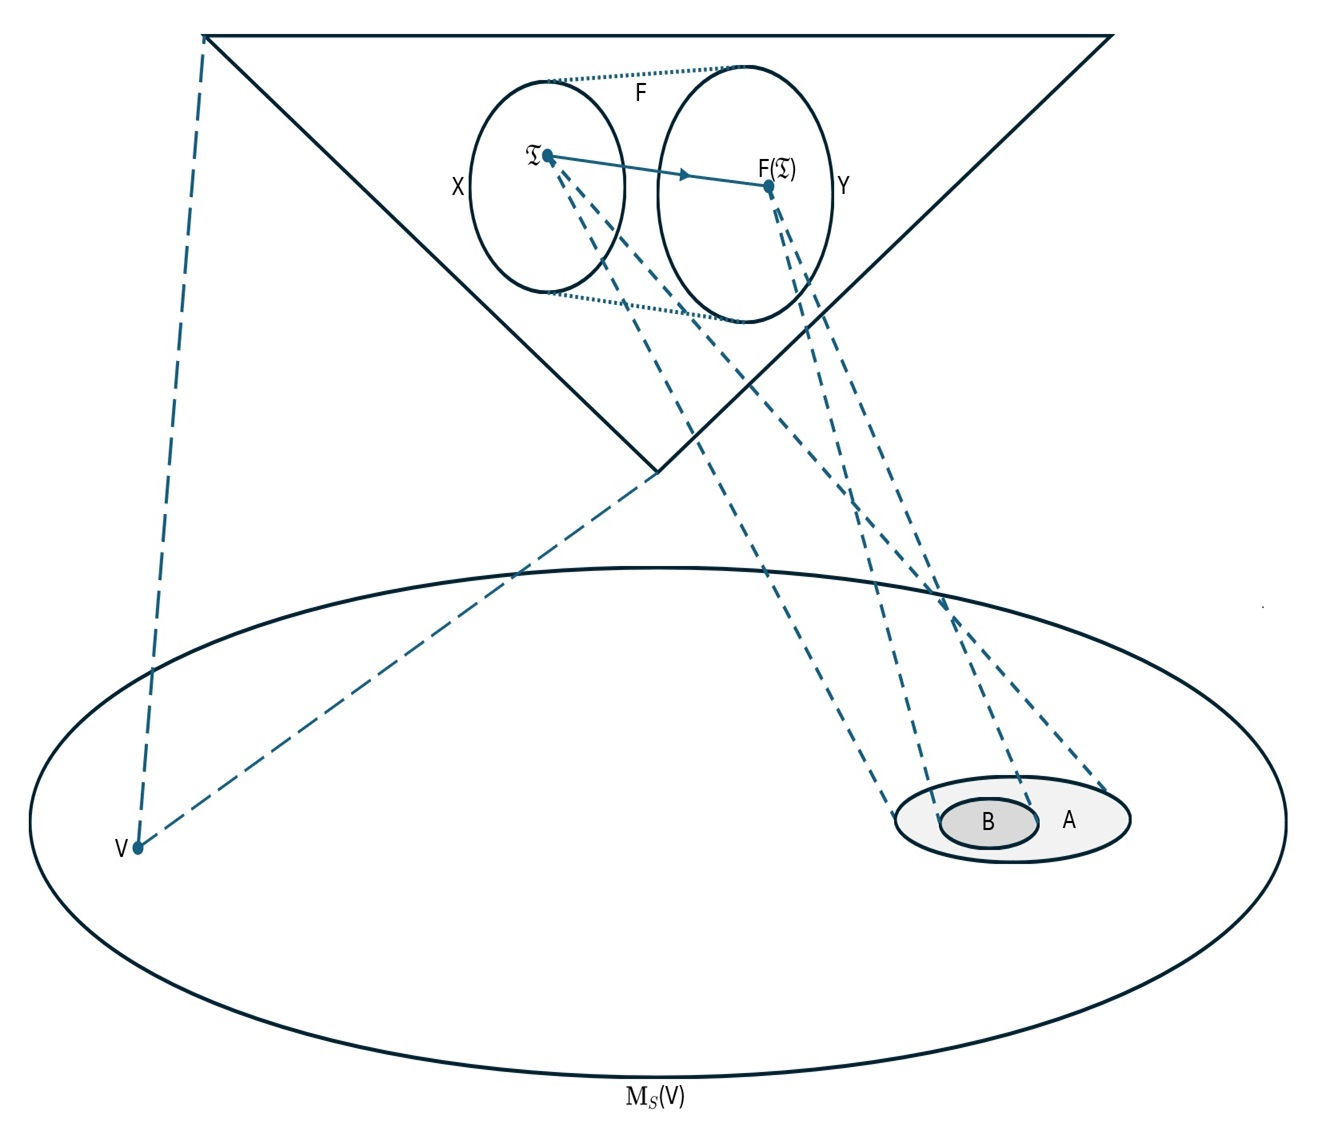
\includegraphics[height = 173pt, width = 280pt]{intuition.jpg}
    \captionsetup{width=0.9\textwidth, format=hang}
    \caption[.]{Visual representation of a function $F$ witnessing $X \leq^M Y$, where $X$ and $Y$ are local method definitions.}
    \label{intuition}
\end{figure}
\end{frame}

\begin{frame}{The Local Method Hierarchy}
\pause{}
\begin{itemize}
    \item We can also define the complexity of a TCI by just looking at its first-order theory.
    \pause{}
    \item For example, a $\Sigma_n$ TCI has a first-order theory containing only $\Sigma_n$ sentences.
    \pause{}
    \item The classes of $\Sigma_n$ and $\Pi_n$ TCIs --- denoted $\mathsf{\Sigma^M_n}$ and $\mathsf{\Pi^M_n}$ respectively --- then form a hierarchy under the relation $\leq^M$, called the local method hierarchy.
\end{itemize}
\end{frame}

\begin{frame}{The Local Method Hierarchy}
\pause{}
\begin{theorem}[L.]
Let $1 \leq n < \omega$. Then for every $\mathcal{T} \in \mathsf{\Pi^M_{n+1}}$ there is $\mathcal{T}' \in \mathsf{\Sigma^M_n}$ such that 
\pause{}
\begin{equation*}
    \mathrm{Eval}^V(\mathcal{T}) = \mathrm{Eval}^V(\mathcal{T}') \text{.}
\end{equation*}
\end{theorem}
\pause{}
\begin{corollary}
$\mathsf{\Pi^M_{n+1}} \leq^M \mathsf{\Sigma^M_n}$ for all $1 \leq n < \omega$.
\end{corollary}
\end{frame}

\begin{frame}{Set Forcing}
\pause{}
\begin{itemize}
    \item There is an obvious way of representing any forcing notion as a $\Pi_2$ TCI.
    \pause{}
    \item Thus set forcing, as a technique of accessing small extensions of $V$, can be represented by a local method definition, denoted $\mathsf{Fg}$.
    \pause{}
    \item We want to see if $\mathsf{Fg}$ fits nicely in the local method hierarchy.
    \pause{}
    \item From what we know so far, $\mathsf{Fg} \leq^M \mathsf{\Sigma^M_1}$.
\end{itemize}
\end{frame}

\begin{frame}{Set Forcing is $\Sigma_1$ (is $\Pi_2$)}
\pause{}
\begin{theorem}[L.]
    $\mathsf{Fg} \equiv^M \mathsf{\Sigma^M_1}$.
\end{theorem}
\pause{}
\begin{proof}[Proof Idea]
    By adapting our framework for constructing forcing notions to the context of TCIs, we associate with each $\Pi_2$ TCI $\mathcal{T}$ a forcing notion $\mathbb{P}(\mathcal{T})$, such that a unique model of $\mathcal{T}$ can be read off every $\mathbb{P}(\mathcal{T})$-generic filter over $V$. 
    \pause{}
    
    \medskip
    This allows us to define a class function witnessing $\mathsf{\Pi^M_2} \leq^M \mathsf{Fg}$.
\end{proof}
\end{frame}

\begin{frame}{Further Results}
\pause{}
\begin{itemize}
    \item We can refine the function witnessing $\mathsf{\Pi^M_2} \leq^M \mathsf{Fg}$ by iteratively pruning the $\mathbb{P}(\mathcal{T})$s of atoms.
    \pause{}
    \item There are analogues of the previous theorem in $V$ pertaining to certain countable $\Pi_2$ TCIs.
    \pause{}
    \begin{itemize}
        \item Essentially, we can define functions $F$ of low complexity taking these TCIs to reals such that every $F(\mathcal{T})$-$1$-generic real codes a model of $\mathcal{T}$.
    \end{itemize}
\end{itemize}
\end{frame}

\begin{frame}{Some Open Questions}
\pause{}
\begin{enumerate}[label=(Q\arabic*)]
    \item What structural properties of $(\mathbf{M}_F(L), \subset)$ also hold for $(\mathbf{M}_S(L), \subset)$?
    \pause{}
    \item For example, is $(\mathbf{M}_S(L), \subset)$ downward directed?
    \pause{}
    \item Are there $m, n < \omega$ for which $\mathsf{\Sigma^M_m} \not\equiv^M \mathsf{\Sigma^M_n}$?
    \pause{}
    \item Is there a TCI $\mathcal{T}$ such that $\{\mathcal{T}\} \not\leq^M \mathsf{Fg}$?
\end{enumerate}
\end{frame}

\section*{}
\begin{frame}{References}
\printbibliography[heading=none]
    
\end{frame}

\section*{}
\begin{frame}
\begin{center}
\Huge Thank You!
\end{center}
\end{frame}

\end{document}
